\documentclass[ctex]{article}
\usepackage{geometry}
\newgeometry{left=3.18cm,right=3.18cm,top=0.20cm,bottom=2.54cm}
\usepackage{graphicx} % Required for inserting images
\usepackage{ctex}
\usepackage{tikz,calc}
\usepackage{amsmath}
\usepackage{float}
\usepackage{physics}
\newcommand{\m}{\mathrm}

\title{粘弹性实验}
\author{物理32   冯家琦   2023011338}
\date{10月10日}
\begin{document}
\maketitle
\begin{abstract}
    本实验使用标准线性固体模型的多重粘弹性过程,并设置应力弛豫条件,探究细线的粘弹性行为,并使我们掌握多重指数项的数据处理方法。实验通过架子来保持应力弛豫条件,并通过合理近似分段进行线性拟合,最终结果与实验数据拟合较好。
\end{abstract}
\section{实验原理}


对于较小外力,材料形变与外力正比(胡克定律)且可逆;对于较大的形变,材料会达到塑性状态,并逐渐变得不可逆。这种情况下,材料内部的分子运动开始不受约束,其行为类似于粘性流体,这种既有弹性性质也有粘性流体的特征称为粘弹性。\par
描述线性粘弹性的唯象模型称为标准线性固体模型,该模型描述粘弹性材料时,分开考虑弹性行为和粘性行为。考虑$n$种粘弹性成分,以及应力弛豫条件($\dv{\epsilon}{t}=0$),可解得:
\begin{equation}
    \sigma(t)=\epsilon\left(E_0+\sum_kE_ke^{-\frac{t}{\tau_k}}\right),k=1,2,…,n
\end{equation}
其中$E_0,E_k$为杨氏模量,$\tau_k$为衰减时间常数,$\epsilon$为应变,$\sigma$为应力,$t$为从施加应变开始记录的时间。
\section{实验仪器及实验步骤}
\subsection{实验仪器}
架子;待测细线; 中心带孔的不锈钢圆柱;塑料螺丝和塑料螺帽;塑料螺丝和塑料螺帽;电子天平,量程为 600 g,分辨力为 0.01 g;计时器;手机支架和手机; 卷尺。

\subsection{实验步骤}
\begin{enumerate}
    \item[A] 剪一根长约 44-44.5 cm 的细线,用塑料螺丝和塑料螺帽将细线的一端固定在不锈钢圆柱上。用电子天平测量中心带孔的不锈钢圆柱和一个塑料螺钉、一个塑料螺帽的总质量$M_0$。将细线的另一端用另一组塑料螺丝和塑料螺帽固定。
     \item[B]用卷尺测量细线没有被拉长的情况下、在两个螺帽之间的长度,作为其初始长度$l_0$。
     \item[C]提前放置好手机支架和手机,并打开手机录像功能。把连接了细线的不锈钢圆柱放在电子天平上,把细线另一端的螺丝头安置在铝型材架子上端的小塑料支架上,细线因此被拉伸。在把细线另一端挂在铝型材架子上端的同时用计时器开始计时,手机记录计时器和电子天平的示数。测量过程约35 分钟。
     \item[D]测量悬挂在架子上被拉长的细线的长度,作为其最终长度。
\end{enumerate}

\section{数据处理}
原长$l_0$,拉伸后长度$l$,总质量$M_0$,截面积$S$,应变$\epsilon$的测量结果见表1。
\begin{table}[htbp]
\centering 
\caption{一些单变量的测量结果}

\begin{tabular}{|c|c|c|c|c|c|}
 \hline   $l_0(m)$&$M_0(g)$&$l(m)$&$\epsilon$&$S(m^2)$  \\ \hline
     44.00&79.36&47.51&0.0795454&0.00000078539815 \\ \hline
\end{tabular}
\end{table}
\par 当$t\rightarrow\infty $,可以直接得到$E_0$,有:
\begin{equation}
    \sigma=E_0\epsilon
\end{equation}
这里计算得到(由表2数据)$E_0=21496875\,$Pa。\\
当$t$很大时,近似有:
\begin{equation}
    \dfrac{\sigma}{\epsilon}=E_0+E_1e^{-\frac{t}{\tau_1}}
\end{equation}
亦即:
\begin{equation}
    \dv{(\sigma/\epsilon)}{t}=-\dfrac{E_1}{\tau_1}e^{-\frac{t}{\tau_1}}
\end{equation}
对$\mathrm{In}\left(-\dv{(\sigma/\epsilon)}{t}\right)$与$t$进行线性拟合可以得到$E_1,\tau_1$。\\
\begin{equation}
    \mathrm{In}\left(-\dv{(\sigma/\epsilon)}{t}\right)=\mathrm{In}\left(\dfrac{E_1}{\tau_1}\right)+\frac{t}{\tau_1}
\end{equation}
近似取$\dv{(\sigma/\epsilon)}{t}(t)=\dfrac{(\sigma/\epsilon)(t+\Delta t)-(\sigma/\epsilon)(t)}{\Delta t}$,且有$F=(M_0-m)g$。\\

实验数据与图像见下方。
\begin{figure}[htbp]
    \centering
    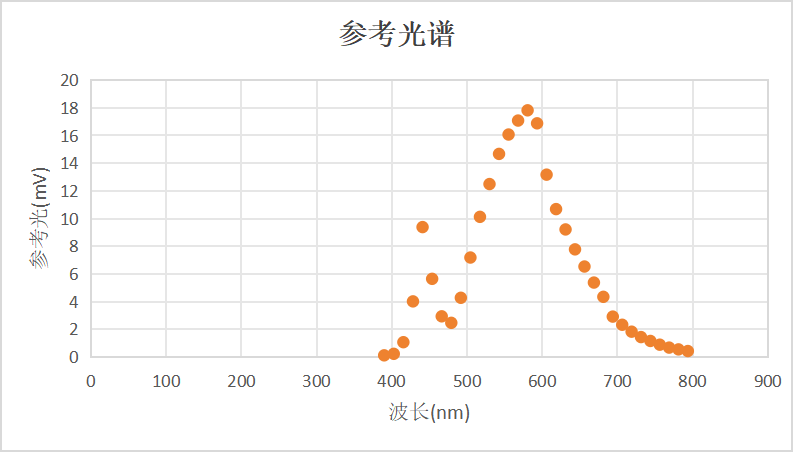
\includegraphics[width=0.8\textwidth,height=0.5\textwidth]{图片1.png}
    \caption{$\mathrm{In}\left(-\dv{(\sigma/\epsilon)}{t}\right)$-$t$图}
\end{figure} 
\begin{table}[H]
    \centering
    \begin{tabular}{|c|c| c|c |c |c|}
\hline
$t(s)$ &$m(g)$&$F(N)$&$\dfrac{\sigma}{\epsilon}(N/m^2)$&$\mathrm{In}\left(-\dv{(\sigma/\epsilon)}{t}\right)$\\
\hline
 0 & 22.06 & 57.3 & 9171690.271 & 7.483521859 \\ \hline
        9 & 22.16 & 57.2 & 9155683.831 & 7.601304895 \\ \hline
        17 & 22.26 & 57.1 & 9139677.391 & 7.378161344 \\ \hline
        27 & 22.36 & 57 & 9123670.95 & 7.629475772 \\ \hline
        34 & 22.45 & 56.91 & 9109265.154 & 7.473471524 \\ \hline
        44 & 22.56 & 56.8 & 9091658.07 & 7.483521859 \\ \hline
        53 & 22.66 & 56.7 & 9075651.63 & 7.483521859 \\ \hline
        62 & 22.76 & 56.6 & 9059645.189 & 7.309168472 \\ \hline
        77 & 22.90  & 56.46 & 9037236.173 & 7.447154215 \\ \hline
        91 & 23.05 & 56.31 & 9013226.513 & 7.195839787 \\ \hline
        109 & 23.2 & 56.16 & 8989216.852 & 7.252998201 \\ \hline
        126 & 23.35 & 56.01 & 8965207.192 & 7.141772566 \\ \hline
        145 & 23.5 & 55.86 & 8941197.531 & 7.090479271 \\ \hline
        165 & 23.65 & 55.71 & 8917187.871 & 7.041689107 \\ \hline
        186 & 23.8 & 55.56 & 8893178.211 & 7.041689107 \\ \hline
        207 & 23.95 & 55.41 & 8869168.55 & 6.908157714 \\ \hline
        231 & 24.1 & 55.26 & 8845158.89 & 6.908157714 \\ \hline
        255 & 24.25 & 55.11 & 8821149.229 & 6.718915715 \\ \hline
        284 & 24.4 & 54.96 & 8797139.569 & 6.718915715 \\ \hline
        313 & 24.55 & 54.81 & 8773129.909 & 6.65222434 \\ \hline
        344 & 24.7 & 54.66 & 8749120.248 & 6.589703983 \\ \hline
        377 & 24.85 & 54.51 & 8725110.588 & 6.475293632 \\ \hline
        414 & 25 & 54.36 & 8701100.928 & 6.372639478 \\ \hline
        455 & 25.15 & 54.21 & 8677091.267 & 6.397332091 \\ \hline
        495 & 25.3 & 54.06 & 8653081.607 & 6.325011429 \\ \hline
        538 & 25.45 & 53.91 & 8629071.946 & 6.194391247 \\ \hline
        587 & 25.6 & 53.76 & 8605062.286 & 6.174188539 \\ \hline
        637 & 25.75 & 53.61 & 8581052.626 & 6.043160277 \\ \hline
        694 & 25.9 & 53.46 & 8557042.965 & 6.043160277 \\ \hline
        751 & 26.05 & 53.31 & 8533033.305 & 5.991866983 \\ \hline
        811 & 26.2 & 53.16 & 8509023.644 & 5.85210504 \\ \hline
        880 & 26.35 & 53.01 & 8485013.984 & 5.85210504 \\ \hline
        949 & 26.5 & 52.86 & 8461004.324 & 5.701064783 \\ \hline
        1056 & 26.7 & 52.66 & 8428991.443 & 5.646505799 \\ \hline
        1169 & 26.9 & 52.46 & 8396978.562 & 5.553612052 \\ \hline
        1293 & 27.1 & 52.26 & 8364965.682 & 5.453912691 \\ \hline
        1430 & 27.3 & 52.06 & 8332952.801 & 5.317647812 \\ \hline
        1587 & 27.5 & 51.86 & 8300939.921 & 5.274027189 \\ \hline
        1751 & 27.7 & 51.66 & 8268927.04 & 5.055773623 \\ \hline
        1955 & 27.9 & 51.46 & 8236914.16 & 5.148146944 \\ \hline
        2141 & 28.1 & 51.26 & 8204901.279 & 11.28551326 \\ \hline
\end{tabular}

    \caption{$t$测量数据}
    \label{tab:my_label}
\end{table}

这里我们取大于900 s的数据来进行拟合。
\par 利用(12)式和Excel程序的linest函数做最小二乘法直线拟合,得到表3。
\begin{table}[htbp]
    \centering
    \begin{tabular}{|c|c|}
    \hline
        $E_1$(Pa) & $\tau_1$(s) \\ \hline
        840492.523712449   &1593.56708837763    \\ \hline
    \end{tabular}
    \caption{$E_1,\tau_1$的拟合结果}
    \label{tab:my_label}
\end{table}
\par  得到$E_1,\tau_1$后,我们也可以利用(10)计算得到$E_0=7991538.026\,$Pa。这里的结果与直接计算结果相差\%5以内。此后我们使用直接计算结果。
\par 当$t$较大时,可略去$E_3$项,近似有:
\begin{equation}
       \mathrm{In}\left(\dfrac{\sigma}{\epsilon}-E_0-E_1e^{-\frac{t}{\tau_1}}\right)=\mathrm{In}E_2-\frac{t}{\tau_2}
\end{equation}
线性拟合得到$E_2,\tau_2$。这里我们取小于900 s的数据进行拟合(见表4及图2)。\\
\begin{figure}[htbp]
    \centering
    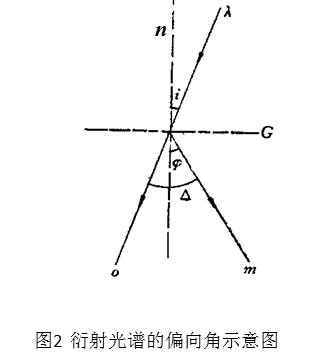
\includegraphics[width=0.8\textwidth,height=0.5\textwidth]{图片2.png}
    \caption{$ \mathrm{In}\left(\dfrac{\sigma}{\epsilon}-E_0-E_1e^{-\frac{t}{\tau_1}}\right)$ - $t$图}
\end{figure} 

可以看出,当取到第二级指数展开的时候就已经呈现出非常好的线性了,因此我们就取到第二种粘性成分
\begin{table}[H]
    \centering
    \begin{tabular}{|c |c| c| c |c |c| c|}
\hline
 $t(s)$ &$\left(\dfrac{\sigma}{\epsilon}-E_0-E_1e^{-\frac{t}{\tau_1}}\right)$ & $ \mathrm{In}\left(\dfrac{\sigma}{\epsilon}-E_0-E_1e^{-\frac{t}{\tau_1}}\right)$\\
\hline
0 & 339659.7216 & 12.73569958 \\ \hline
        9 & 328386.749 & 12.70194731 \\ \hline
        17 & 316565.4514 & 12.6652853 \\ \hline
        27 & 305760.9804 & 12.63055897 \\ \hline
        34 & 294977.1884 & 12.5946533 \\ \hline
        44 & 282516.8743 & 12.55149356 \\ \hline
        53 & 271114.9939 & 12.51029834 \\ \hline
        62 & 259687.1817 & 12.46723304 \\ \hline
        77 & 244851.982 & 12.40840915 \\ \hline
        91 & 227847.1852 & 12.33643044 \\ \hline
        109 & 212753.8232 & 12.26789102 \\ \hline
        126 & 197073.1367 & 12.19133019 \\ \hline
        145 & 182267.7848 & 12.11323223 \\ \hline
        165 & 167829.0406 & 12.03070113 \\ \hline
        186 & 153740.3987 & 11.94302074 \\ \hline
        207 & 139521.8757 & 11.84597668 \\ \hline
        231 & 126545.2286 & 11.74835506 \\ \hline
        255 & 113403.6636 & 11.63870898 \\ \hline
        284 & 102309.766 & 11.53576041 \\ \hline
        313 & 90982.95134 & 11.41842742 \\ \hline
        344 & 80278.00004 & 11.29325089 \\ \hline
        377 & 70149.87822 & 11.15838935 \\ \hline
        414 & 61366.32418 & 11.0246165 \\ \hline
        455 & 53821.01315 & 10.89341925 \\ \hline
        495 & 45471.02596 & 10.72483061 \\ \hline
        538 & 37862.8429 & 10.54172551 \\ \hline
        587 & 32011.60762 & 10.37385385 \\ \hline
        637 & 25964.27469 & 10.16447682 \\ \hline
        694 & 21755.85859 & 9.987638361 \\ \hline
        751 & 16851.69401 & 9.732206466 \\ \hline
        811 & 12228.30312 & 9.411508472 \\ \hline
        880 & 9628.916492 & 9.172525985 \\ \hline
\end{tabular}

    \caption{$t$较小时的数据}
    \label{tab:my_label}
\end{table}
\par 利用(13)式和Excel程序的linest函数做最小二乘法直线拟合,得到表5。
\begin{table}[htbp]
    \centering
    \begin{tabular}{|c|c|}
    \hline
        $E_2$ (Pa)& $\tau_2$ (s)\\ \hline
         365107.124  &239.242863325576   \\ \hline
    \end{tabular}
    \caption{$E_2,\tau_2$的拟合结果}
    \label{tab:my_label}
\end{table}

\begin{figure}[htbp]
    \centering
    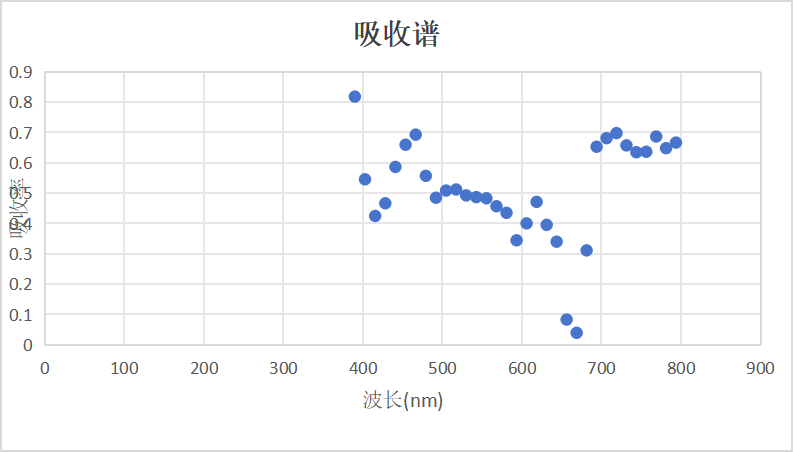
\includegraphics[width=0.8\textwidth,height=0.5\textwidth]{图片3.png}
    \caption{最终的拟合结果,黄色点为测得的力,蓝色点为拟合的数据}
\end{figure} 

\section{分析讨论}
\begin{enumerate}
    \item 本实验学会了处理多重指数项的数据,通过合理近似分段选取数据进行线性拟合,最终得到了较好的结果。
    \item 对$E_1,\tau_1$线性拟合时线性并不很好($r^2\approx0.89$),这主要是因为时间较长时$m$测量值反复波动所致。但$E_2,E_3,\tau_2,\tau_3$拟合线性很好($r^2>0.99$),并且最终拟合结果很好,可见此方法比较有效。
    \item 最终算得的$\tau_1,\tau_2$和所选取的数据时间段的数量级一致,可见这样分段选取是合理的。 如果进一步考虑三种粘弹性成分可能会导致不精确,因为理论上第四种将为1 s量级,已经与计时器分度值接近,可能需要更加精确的计时器。
\end{enumerate}
\end{document}
